\documentclass[aspectratio=169,11pt]{beamer}

\usepackage[utf8]{inputenc}
\usepackage[T1]{fontenc}
\usepackage[english]{babel}
\usepackage{amsmath,amssymb}
\usepackage{graphicx}
\usepackage{hyperref}

\usetheme{default}
\definecolor{upblue}{RGB}{0,62,116}
\definecolor{upgold}{RGB}{214,158,46}
\setbeamercolor{structure}{fg=upblue}
\setbeamercolor{frametitle}{fg=white,bg=upblue}
\setbeamercolor{alerted text}{fg=upgold!80!black}
\setbeamertemplate{navigation symbols}{}
\setbeamertemplate{footline}[frame number]
\setbeamerfont{frametitle}{size=\large,series=\bfseries}

\title{Human--AI Productivity Paradoxes}
\subtitle{Aouad, Lykouris \& Zhong (2026) --- Proposition 2.1}
\author{John Barraza}
\institute{Artificial Intelligence and Economic Modeling\\Universidad del Pacífico}
\date{Repository 1 --- August 2026}

\newcommand{\repolink}{https://github.com/johnbarraza/ai-01-aouad}

\begin{document}

\begin{frame}[plain]
  \titlepage
  \vspace{-0.8em}
  \begin{center}
    \small\href{\repolink}{\texttt{github.com/johnbarraza/ai-01-aouad}}
  \end{center}
\end{frame}

\begin{frame}{1. The paper}
  \textbf{Question.} Can AI reduce human effort while still increasing output?

  \medskip
  \textbf{Single mechanism.} Skill, effort, and AI are perfect substitutes:
  \[
    x=s+e+a.
  \]

  \textbf{Agent's problem.}
  \[
    \max_{e\geq0}\;p(s+e+a)-\gamma e.
  \]

  \begin{block}{Economic intuition}
    Skill and AI each replace costly effort one for one. The constraint
    $e\geq0$ creates the interior-versus-corner split.
  \end{block}
\end{frame}

\begin{frame}{2. Proposition 2.1 --- result and conditions}
  \small
  \textbf{Conditions:} $s>0$, $a\geq0$, $\gamma>0$; $p:\mathbb R_+\to\mathbb R_+$
  is weakly increasing, weakly concave, continuous, and twice differentiable;
  and
  \[
    \limsup_{x\to\infty}\frac{p(x)}{x}<\gamma.
  \]

  Define the critical input with the \alert{largest-maximizer tie-break}:
  \[
    x^*=\max\arg\max_{x\geq0}\{p(x)-\gamma x\}.
  \]

  \textbf{Then}
  \[
    e^*(s,a)=(x^*-s-a)_+,
    \qquad
    p^*(s,a)=\max\{p(x^*),p(s+a)\}.
  \]

  \begin{block}{One-sentence intuition}
    The worker tops total input up to $x^*$; once $s+a$ reaches that target,
    effort falls to zero.
  \end{block}
\end{frame}

\begin{frame}{3. What I did}
  \begin{enumerate}
    \item Rewrote the choice using total input:
      \[
        \max_{x\geq s+a}\{p(x)-\gamma x\}+\gamma(s+a).
      \]
    \item Verified the two feasible cases instead of assuming an interior FOC:
      \[
      x^{\mathrm{opt}}=
      \begin{cases}
        x^*, & s+a\leq x^*,\\
        s+a, & s+a>x^*.
      \end{cases}
      \]
    \item Numerically audited the formula for
      $p(x)=10(1-e^{-0.4x})$ in \texttt{verify\_proposition.py}.
    \item Checked possible extensions: convex effort cost is already in
      Appendix D; a two-period non-myopic agent remains a tractable candidate.
  \end{enumerate}
\end{frame}

\begin{frame}{4. Where I did not believe the AI}
  \begin{columns}[T,onlytextwidth]
    \begin{column}{0.57\textwidth}
      \small
      \textbf{AI claim.} The first-order condition
      $p'(s+e+a)=\gamma$ proves the result.

      \medskip
      \textbf{Verdict: \alert{incomplete}.}
      \begin{itemize}
        \item It starts by assuming an interior optimum.
        \item It misses the corner $e=0$.
        \item It does not handle a flat maximizing set or justify the paper's
          largest-maximizer tie-break.
      \end{itemize}

      \textbf{My check.} I derived the feasible set $x\geq s+a$ and verified
      both cases directly from concavity.
    \end{column}
    \begin{column}{0.40\textwidth}
      \centering
      \IfFileExists{hand/prop-2-1-case-split.jpg}{%
        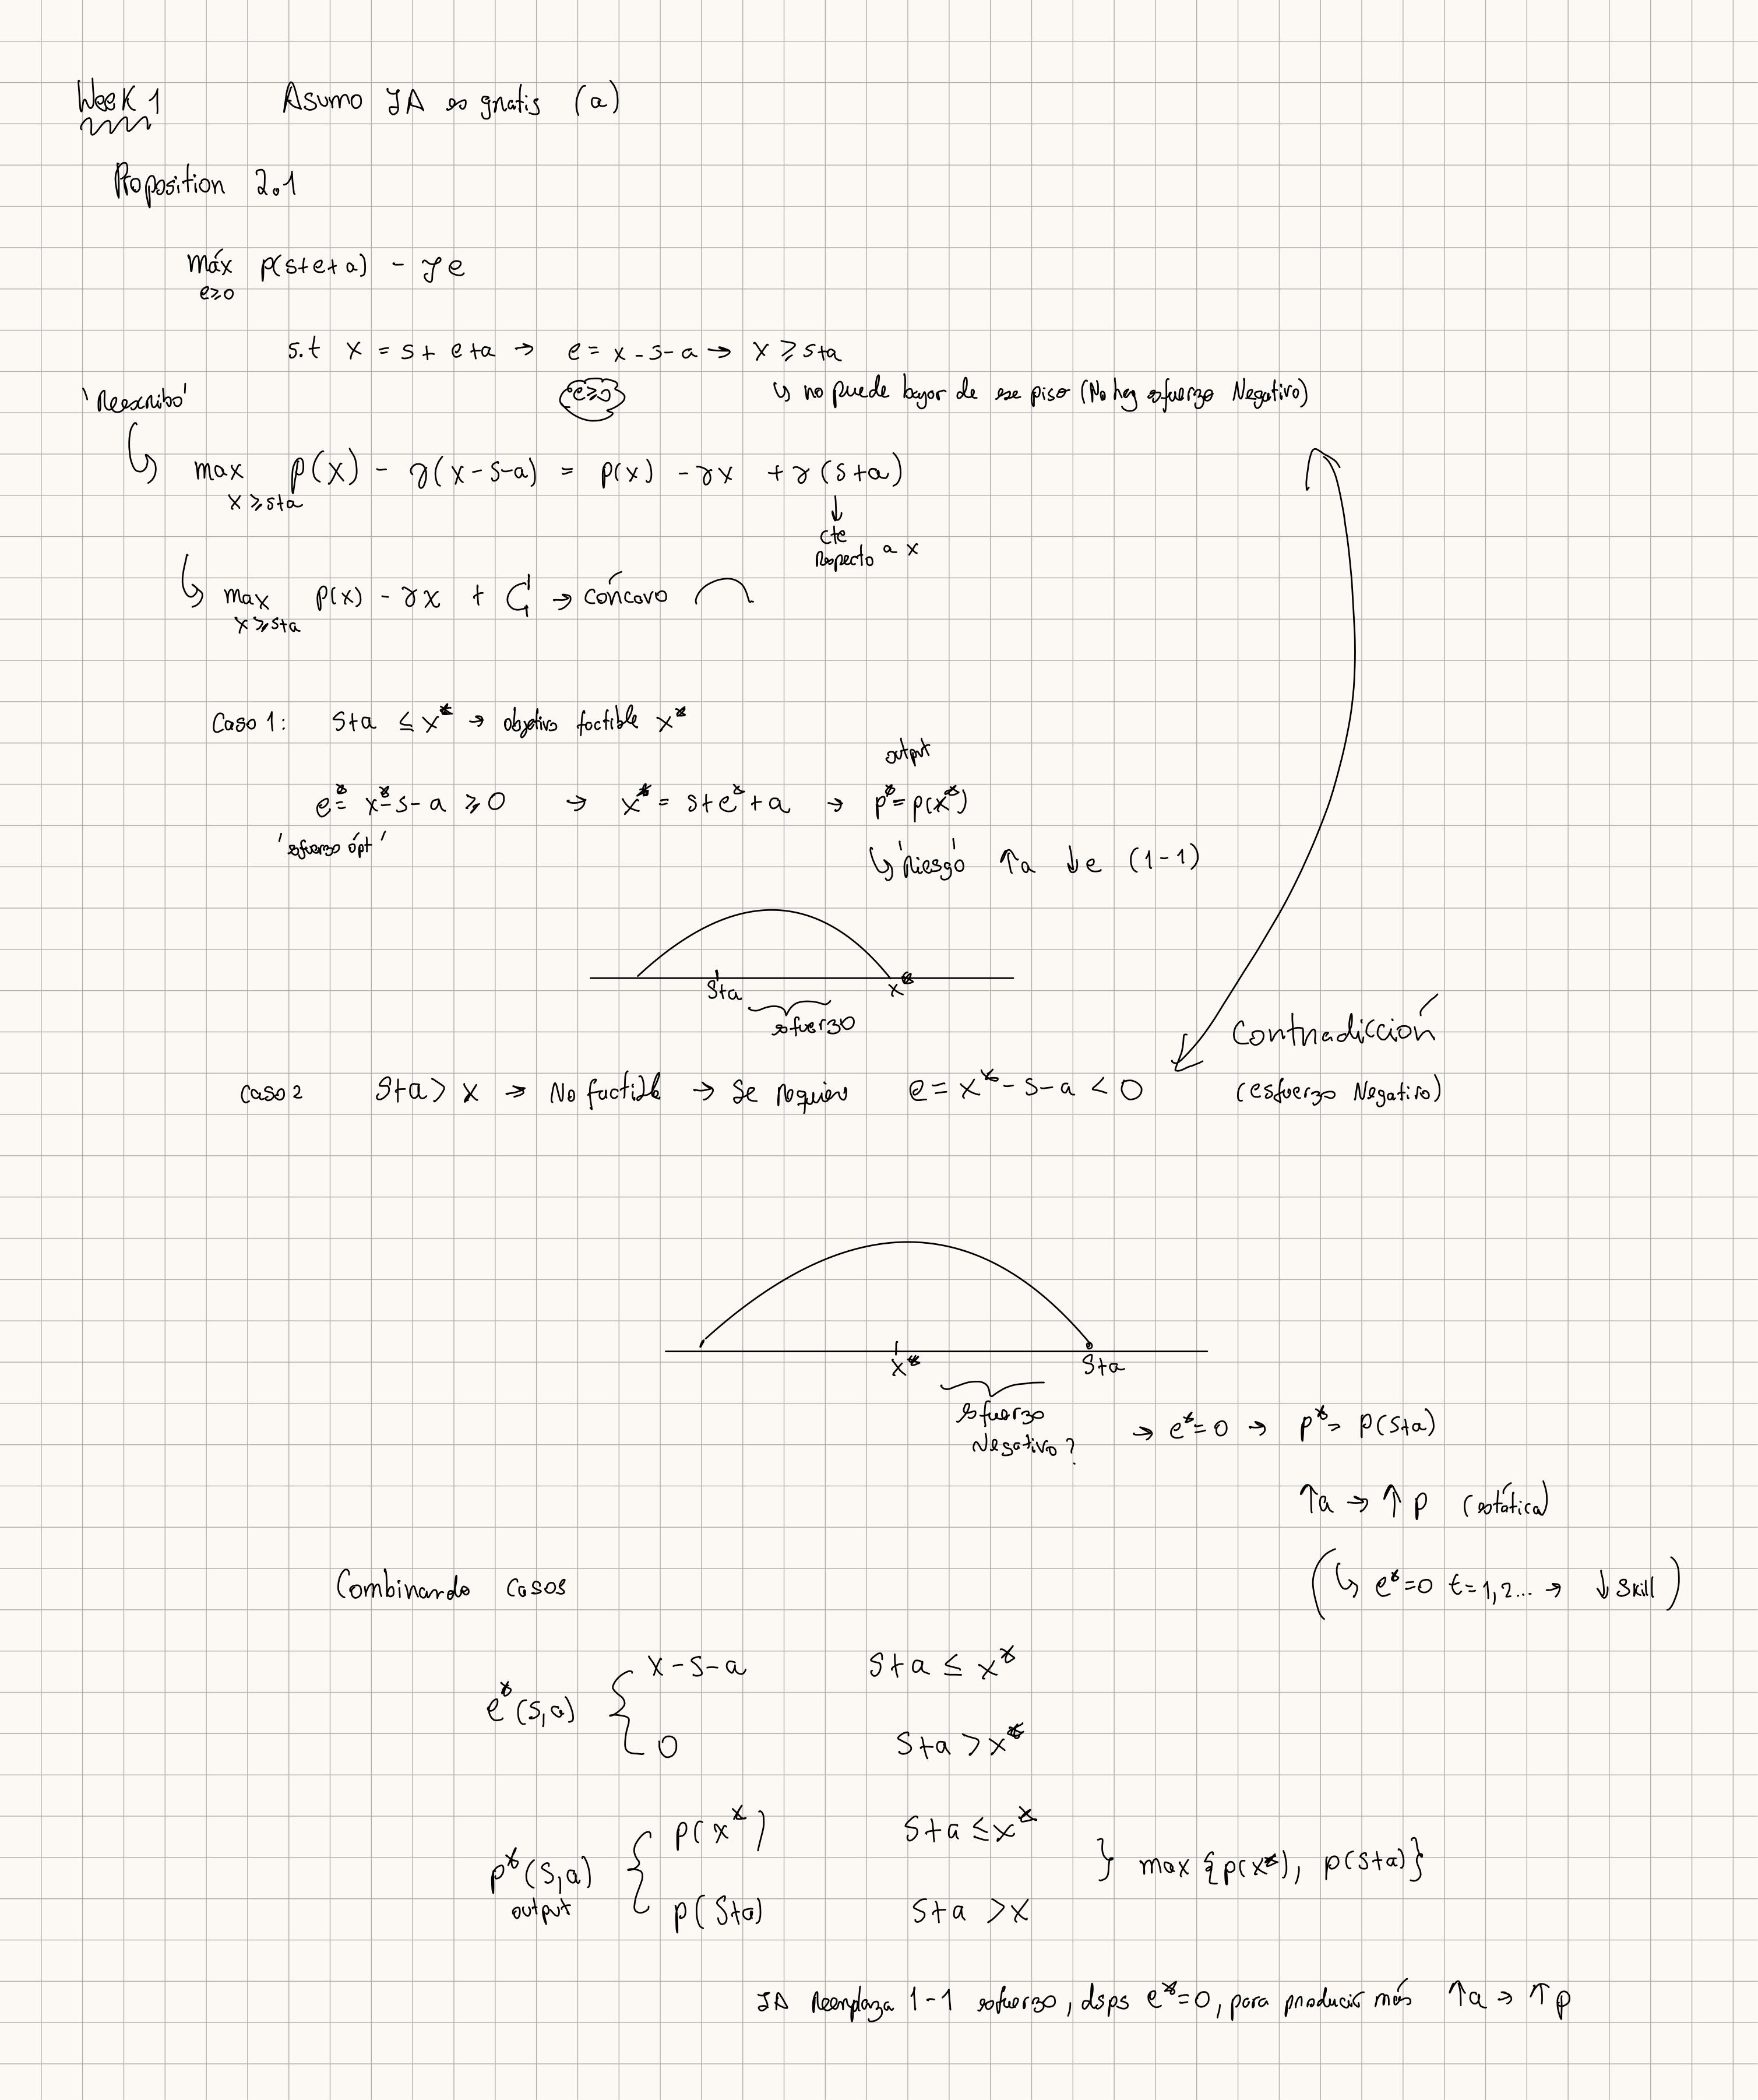
\includegraphics[width=\textwidth,height=0.57\textheight,keepaspectratio]
          {hand/prop-2-1-case-split.jpg}%
      }{%
        \fbox{\parbox[c][0.47\textheight][c]{0.88\textwidth}{\centering
          \textbf{Handwritten photo pending}\\[0.8em]
          Add\\
          \texttt{hand/prop-2-1-}\\
          \texttt{case-split.jpg}\\[0.8em]
          before merge.}}
      }
    \end{column}
  \end{columns}
\end{frame}

\end{document}
